\documentclass[border=5pt]{standalone}
\usepackage[T1]{fontenc}
\usepackage{lmodern}
\usepackage{pgfplots}
\usepgfplotslibrary{groupplots}
\pgfplotsset{compat=1.18}
\begin{document}
\sffamily
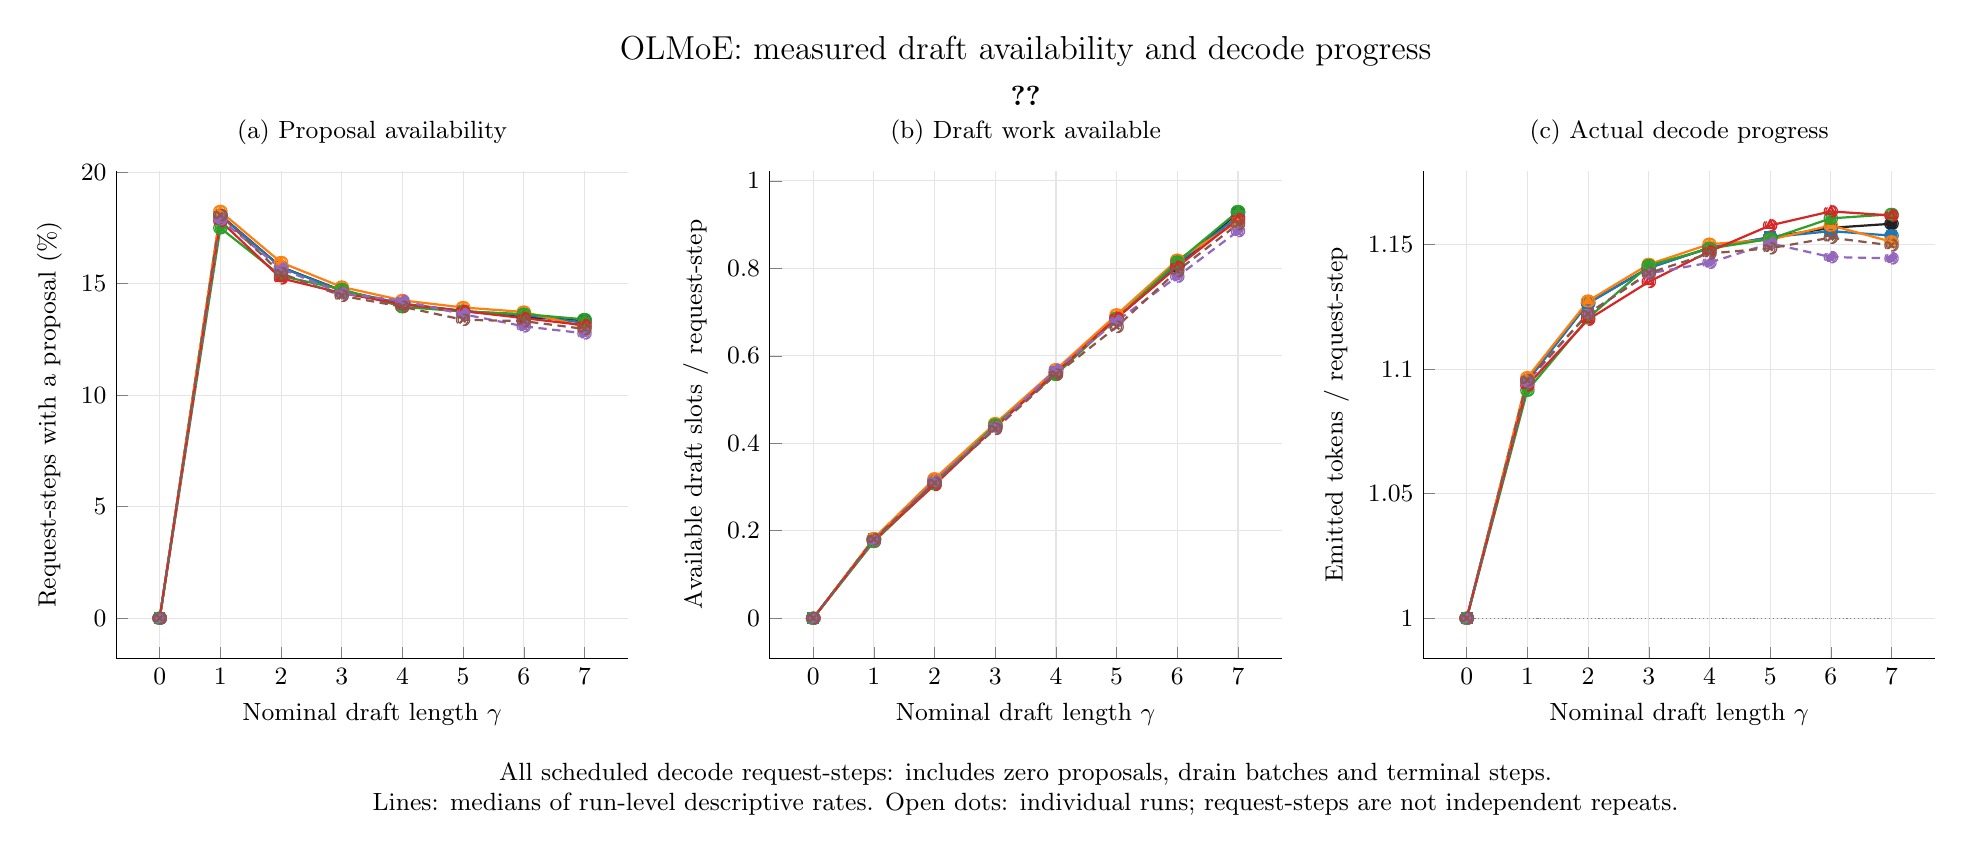
\begin{tikzpicture}
\definecolor{series0}{HTML}{222222}
\definecolor{series1}{HTML}{1f77b4}
\definecolor{series2}{HTML}{ff7f0e}
\definecolor{series3}{HTML}{2ca02c}
\definecolor{series4}{HTML}{d62728}
\definecolor{series5}{HTML}{9467bd}
\definecolor{series6}{HTML}{8c564b}
\definecolor{series7}{HTML}{e377c2}
\begin{groupplot}[group style={group size=3 by 1,horizontal sep=1.8cm},width=6.5cm,height=6.2cm,scale only axis,grid=major,grid style={gray!20},axis lines*=left,tick label style={font=\small},label style={font=\small},title style={font=\small},unbounded coords=jump]
\nextgroupplot[title={(a) Proposal availability},xlabel={Nominal draft length $\gamma$},ylabel={Request-steps with a proposal (\%)},xtick={0,1,2,3,4,5,6,7},xticklabels={0,1,2,3,4,5,6,7},scaled y ticks=false,yticklabel style={/pgf/number format/fixed,/pgf/number format/precision=2},legend columns=7,legend to name=sharedlegend,legend style={draw=none,font=\small,/tikz/every even column/.append style={column sep=8pt}}]
\addplot+[color=series0,mark=*,mark size=1.7pt,mark options={fill=series0,draw=series0},line width=0.8pt] coordinates {(0,0) (1,18.0727762803) (2,15.744975745) (3,14.6926747123) (4,14.0898812889) (5,13.7730496454) (6,13.4908211185) (7,13.367535984)};
\addlegendentry{$B=1$}
\addplot+[only marks,forget plot,color=series0,mark=o,mark size=2.1pt,mark options={fill=white,line width=0.45pt}] coordinates {(-0.014,0) (0.014,0) (0.986,18.0727762803) (1.014,18.0727762803) (1.986,15.744975745) (2.014,15.744975745) (2.986,14.6926747123) (3.014,14.6926747123) (3.986,14.0898812889) (4.014,14.0898812889) (4.986,13.7730496454) (5.014,13.7730496454) (5.986,13.4908211185) (6.014,13.4908211185) (6.986,13.367535984) (7.014,13.367535984)};
\addplot+[color=series1,mark=square*,mark size=1.7pt,mark options={fill=series1,draw=series1},line width=0.8pt] coordinates {(0,0) (1,18.0568656515) (2,15.7289356984) (3,14.6786415942) (4,14.104013567) (5,13.7730496454) (6,13.6034115139) (7,13.2415554925)};
\addlegendentry{$B=2$}
\addplot+[only marks,forget plot,color=series1,mark=o,mark size=2.1pt,mark options={fill=white,line width=0.45pt}] coordinates {(-0.014,0) (0.014,0) (0.986,18.0568656515) (1.014,18.0568656515) (1.986,15.7289356984) (2.014,15.7289356984) (2.986,14.6786415942) (3.014,14.6786415942) (3.986,14.104013567) (4.014,14.104013567) (4.986,13.7730496454) (5.014,13.7730496454) (5.986,13.6034115139) (6.014,13.6034115139) (6.986,13.2415554925) (7.014,13.2415554925)};
\addplot+[color=series2,mark=triangle*,mark size=1.7pt,mark options={fill=series2,draw=series2},line width=0.8pt] coordinates {(0,0) (1,18.2406907717) (2,15.9500693481) (3,14.8517633834) (4,14.2493278619) (5,13.9314058957) (6,13.7302378579) (7,13.0718028608)};
\addlegendentry{$B=4$}
\addplot+[only marks,forget plot,color=series2,mark=o,mark size=2.1pt,mark options={fill=white,line width=0.45pt}] coordinates {(-0.014,0) (0.014,0) (0.986,18.2406907717) (1.014,18.2406907717) (1.986,15.9500693481) (2.014,15.9500693481) (2.986,14.8517633834) (3.014,14.8517633834) (3.986,14.2493278619) (4.014,14.2493278619) (4.986,13.9314058957) (5.014,13.9314058957) (5.986,13.7302378579) (6.014,13.7302378579) (6.986,13.0718028608) (7.014,13.0718028608)};
\addplot+[color=series3,mark=diamond*,mark size=1.7pt,mark options={fill=series3,draw=series3},line width=0.8pt] coordinates {(0,0) (1,17.4969786491) (2,15.3432588916) (3,14.7471910112) (4,13.9587454083) (5,13.7510632265) (6,13.6350656768) (7,13.3971975979)};
\addlegendentry{$B=8$}
\addplot+[only marks,forget plot,color=series3,mark=o,mark size=2.1pt,mark options={fill=white,line width=0.45pt}] coordinates {(-0.014,0) (0.014,0) (0.986,17.4969786491) (1.014,17.4969786491) (1.986,15.3432588916) (2.014,15.3432588916) (2.986,14.7471910112) (3.014,14.7471910112) (3.986,13.9587454083) (4.014,13.9587454083) (4.986,13.7510632265) (5.014,13.7510632265) (5.986,13.6350656768) (6.014,13.6350656768) (6.986,13.3971975979) (7.014,13.3971975979)};
\addplot+[color=series4,mark=triangle,mark size=1.7pt,mark options={fill=series4,draw=series4},line width=0.8pt] coordinates {(0,0) (1,17.8124579578) (2,15.2383576743) (3,14.5789694177) (4,14.0719830628) (5,13.7729668138) (6,13.4535566051) (7,13.1342003716)};
\addlegendentry{$B=16$}
\addplot+[only marks,forget plot,color=series4,mark=o,mark size=2.1pt,mark options={fill=white,line width=0.45pt}] coordinates {(-0.014,0) (0.014,0) (0.986,17.8124579578) (1.014,17.8124579578) (1.986,15.2383576743) (2.014,15.2383576743) (2.986,14.5789694177) (3.014,14.5789694177) (3.986,14.0719830628) (4.014,14.0719830628) (4.986,13.7729668138) (5.014,13.7729668138) (5.986,13.4535566051) (6.014,13.4535566051) (6.986,13.1342003716) (7.014,13.1342003716)};
\addplot+[color=series5,mark=pentagon*,mark size=1.7pt,mark options={fill=series5,draw=series5},line width=0.8pt] coordinates {(0,0) (1,17.8879310345) (2,15.6724661696) (3,14.5658263305) (4,14.2274708281) (5,13.6305732484) (6,13.0863501902) (7,12.7710504083)};
\addlegendentry{$B=32$}
\addplot+[only marks,forget plot,color=series5,mark=o,mark size=2.1pt,mark options={fill=white,line width=0.45pt}] coordinates {(-0.014,0) (0.014,0) (0.986,17.8879310345) (1.014,17.8879310345) (1.986,15.6724661696) (2.014,15.6724661696) (2.986,14.5658263305) (3.014,14.5658263305) (3.986,14.2274708281) (4.014,14.2274708281) (4.986,13.6305732484) (5.014,13.6305732484) (5.986,13.0863501902) (6.014,13.0863501902) (6.986,12.7710504083) (7.014,12.7710504083)};
\addplot+[color=series6,mark=x,mark size=1.7pt,mark options={fill=series6,draw=series6},line width=0.8pt] coordinates {(0,0) (1,18.0752122928) (2,15.4632058539) (3,14.4558061353) (4,13.9633286319) (5,13.3813762894) (6,13.3172599631) (7,12.9702970297)};
\addlegendentry{$B=64$}
\addplot+[only marks,forget plot,color=series6,mark=o,mark size=2.1pt,mark options={fill=white,line width=0.45pt}] coordinates {(-0.014,0) (0.014,0) (0.986,18.0752122928) (1.014,18.0752122928) (1.986,15.4632058539) (2.014,15.4632058539) (2.986,14.4558061353) (3.014,14.4558061353) (3.986,13.9633286319) (4.014,13.9633286319) (4.986,13.3813762894) (5.014,13.3813762894) (5.986,13.3172599631) (6.014,13.3172599631) (6.986,12.9702970297) (7.014,12.9702970297)};
\nextgroupplot[title={(b) Draft work available},xlabel={Nominal draft length $\gamma$},ylabel={Available draft slots / request-step},xtick={0,1,2,3,4,5,6,7},xticklabels={0,1,2,3,4,5,6,7},scaled y ticks=false,yticklabel style={/pgf/number format/fixed,/pgf/number format/precision=2}]
\addplot+[color=series0,mark=*,mark size=1.7pt,mark options={fill=series0,draw=series0},line width=0.8pt] coordinates {(0,0) (1,0.180727762803) (2,0.3148995149) (3,0.440359247825) (4,0.562464669305) (5,0.686524822695) (6,0.805180019923) (7,0.928031922474)};
\addplot+[only marks,forget plot,color=series0,mark=o,mark size=2.1pt,mark options={fill=white,line width=0.45pt}] coordinates {(-0.014,0) (0.014,0) (0.986,0.180727762803) (1.014,0.180727762803) (1.986,0.3148995149) (2.014,0.3148995149) (2.986,0.440359247825) (3.014,0.440359247825) (3.986,0.562464669305) (4.014,0.562464669305) (4.986,0.686524822695) (5.014,0.686524822695) (5.986,0.805180019923) (6.014,0.805180019923) (6.986,0.928031922474) (7.014,0.928031922474)};
\addplot+[color=series1,mark=square*,mark size=1.7pt,mark options={fill=series1,draw=series1},line width=0.8pt] coordinates {(0,0) (1,0.180568656515) (2,0.314578713969) (3,0.440078585462) (4,0.56302996043) (5,0.685957446809) (6,0.811513859275) (7,0.918961112688)};
\addplot+[only marks,forget plot,color=series1,mark=o,mark size=2.1pt,mark options={fill=white,line width=0.45pt}] coordinates {(-0.014,0) (0.014,0) (0.986,0.180568656515) (1.014,0.180568656515) (1.986,0.314578713969) (2.014,0.314578713969) (2.986,0.440078585462) (3.014,0.440078585462) (3.986,0.56302996043) (4.014,0.56302996043) (4.986,0.685957446809) (5.014,0.685957446809) (5.986,0.811513859275) (6.014,0.811513859275) (6.986,0.918961112688) (7.014,0.918961112688)};
\addplot+[color=series2,mark=triangle*,mark size=1.7pt,mark options={fill=series2,draw=series2},line width=0.8pt] coordinates {(0,0) (1,0.182406907717) (2,0.319001386963) (3,0.445271884221) (4,0.568699589642) (5,0.69387755102) (6,0.819114086312) (7,0.906953689279)};
\addplot+[only marks,forget plot,color=series2,mark=o,mark size=2.1pt,mark options={fill=white,line width=0.45pt}] coordinates {(-0.014,0) (0.014,0) (0.986,0.182406907717) (1.014,0.182406907717) (1.986,0.319001386963) (2.014,0.319001386963) (2.986,0.445271884221) (3.014,0.445271884221) (3.986,0.568699589642) (4.014,0.568699589642) (4.986,0.69387755102) (5.014,0.69387755102) (5.986,0.819114086312) (6.014,0.819114086312) (6.986,0.906953689279) (7.014,0.906953689279)};
\addplot+[color=series3,mark=diamond*,mark size=1.7pt,mark options={fill=series3,draw=series3},line width=0.8pt] coordinates {(0,0) (1,0.174969786491) (2,0.306865177833) (3,0.441994382022) (4,0.557078270698) (5,0.685284944712) (6,0.814962878355) (7,0.930368887618)};
\addplot+[only marks,forget plot,color=series3,mark=o,mark size=2.1pt,mark options={fill=white,line width=0.45pt}] coordinates {(-0.014,0) (0.014,0) (0.986,0.174969786491) (1.014,0.174969786491) (1.986,0.306865177833) (2.014,0.306865177833) (2.986,0.441994382022) (3.014,0.441994382022) (3.986,0.557078270698) (4.014,0.557078270698) (4.986,0.685284944712) (5.014,0.685284944712) (5.986,0.814962878355) (6.014,0.814962878355) (6.986,0.930368887618) (7.014,0.930368887618)};
\addplot+[color=series4,mark=triangle,mark size=1.7pt,mark options={fill=series4,draw=series4},line width=0.8pt] coordinates {(0,0) (1,0.178124579578) (2,0.304767153486) (3,0.437089791929) (4,0.561891319689) (5,0.686511892893) (6,0.8034921998) (7,0.912533943118)};
\addplot+[only marks,forget plot,color=series4,mark=o,mark size=2.1pt,mark options={fill=white,line width=0.45pt}] coordinates {(-0.014,0) (0.014,0) (0.986,0.178124579578) (1.014,0.178124579578) (1.986,0.304767153486) (2.014,0.304767153486) (2.986,0.437089791929) (3.014,0.437089791929) (3.986,0.561891319689) (4.014,0.561891319689) (4.986,0.686511892893) (5.014,0.686511892893) (5.986,0.8034921998) (6.014,0.8034921998) (6.986,0.912533943118) (7.014,0.912533943118)};
\addplot+[color=series5,mark=pentagon*,mark size=1.7pt,mark options={fill=series5,draw=series5},line width=0.8pt] coordinates {(0,0) (1,0.178879310345) (2,0.313449323391) (3,0.436694677871) (4,0.568114719528) (5,0.679263977353) (6,0.781377658825) (7,0.885384398761)};
\addplot+[only marks,forget plot,color=series5,mark=o,mark size=2.1pt,mark options={fill=white,line width=0.45pt}] coordinates {(-0.014,0) (0.014,0) (0.986,0.178879310345) (1.014,0.178879310345) (1.986,0.313449323391) (2.014,0.313449323391) (2.986,0.436694677871) (3.014,0.436694677871) (3.986,0.568114719528) (4.014,0.568114719528) (4.986,0.679263977353) (5.014,0.679263977353) (5.986,0.781377658825) (6.014,0.781377658825) (6.986,0.885384398761) (7.014,0.885384398761)};
\addplot+[color=series6,mark=x,mark size=1.7pt,mark options={fill=series6,draw=series6},line width=0.8pt] coordinates {(0,0) (1,0.180752122928) (2,0.309264117079) (3,0.432973805855) (4,0.557263751763) (5,0.666384061043) (6,0.79435541058) (7,0.901414427157)};
\addplot+[only marks,forget plot,color=series6,mark=o,mark size=2.1pt,mark options={fill=white,line width=0.45pt}] coordinates {(-0.014,0) (0.014,0) (0.986,0.180752122928) (1.014,0.180752122928) (1.986,0.309264117079) (2.014,0.309264117079) (2.986,0.432973805855) (3.014,0.432973805855) (3.986,0.557263751763) (4.014,0.557263751763) (4.986,0.666384061043) (5.014,0.666384061043) (5.986,0.79435541058) (6.014,0.79435541058) (6.986,0.901414427157) (7.014,0.901414427157)};
\nextgroupplot[title={(c) Actual decode progress},xlabel={Nominal draft length $\gamma$},ylabel={Emitted tokens / request-step},xtick={0,1,2,3,4,5,6,7},xticklabels={0,1,2,3,4,5,6,7},scaled y ticks=false,yticklabel style={/pgf/number format/fixed,/pgf/number format/precision=2}]
\addplot+[color=series0,mark=*,mark size=1.7pt,mark options={fill=series0,draw=series0},line width=0.8pt] coordinates {(0,1) (1,1.09541778976) (2,1.12654192654) (3,1.14061184395) (4,1.14867156586) (5,1.15290780142) (6,1.15668137185) (7,1.15832977056)};
\addplot+[only marks,forget plot,color=series0,mark=o,mark size=2.1pt,mark options={fill=white,line width=0.45pt}] coordinates {(-0.014,1) (0.014,1) (0.986,1.09541778976) (1.014,1.09541778976) (1.986,1.12654192654) (2.014,1.12654192654) (2.986,1.14061184395) (3.014,1.14061184395) (3.986,1.14867156586) (4.014,1.14867156586) (4.986,1.15290780142) (5.014,1.15290780142) (5.986,1.15668137185) (6.014,1.15668137185) (6.986,1.15832977056) (7.014,1.15832977056)};
\addplot+[color=series1,mark=square*,mark size=1.7pt,mark options={fill=series1,draw=series1},line width=0.8pt] coordinates {(0,1) (1,1.09527017922) (2,1.12638580931) (3,1.14061184395) (4,1.14867156586) (5,1.15290780142) (6,1.15536602701) (7,1.15356230485)};
\addplot+[only marks,forget plot,color=series1,mark=o,mark size=2.1pt,mark options={fill=white,line width=0.45pt}] coordinates {(-0.014,1) (0.014,1) (0.986,1.09527017922) (1.014,1.09527017922) (1.986,1.12638580931) (2.014,1.12638580931) (2.986,1.14061184395) (3.014,1.14061184395) (3.986,1.14867156586) (4.014,1.14867156586) (4.986,1.15290780142) (5.014,1.15290780142) (5.986,1.15536602701) (6.014,1.15536602701) (6.986,1.15356230485) (7.014,1.15356230485)};
\addplot+[color=series2,mark=triangle*,mark size=1.7pt,mark options={fill=series2,draw=series2},line width=0.8pt] coordinates {(0,1) (1,1.09660010793) (2,1.12732316227) (3,1.14205423634) (4,1.15013442762) (5,1.15192743764) (6,1.1576698476) (7,1.15111174055)};
\addplot+[only marks,forget plot,color=series2,mark=o,mark size=2.1pt,mark options={fill=white,line width=0.45pt}] coordinates {(-0.014,1) (0.014,1) (0.986,1.09660010793) (1.014,1.09660010793) (1.986,1.12732316227) (2.014,1.12732316227) (2.986,1.14205423634) (3.014,1.14205423634) (3.986,1.15013442762) (4.014,1.15013442762) (4.986,1.15192743764) (5.014,1.15192743764) (5.986,1.1576698476) (6.014,1.1576698476) (6.986,1.15111174055) (7.014,1.15111174055)};
\addplot+[color=series3,mark=diamond*,mark size=1.7pt,mark options={fill=series3,draw=series3},line width=0.8pt] coordinates {(0,1) (1,1.09144621995) (2,1.12048524952) (3,1.14157303371) (4,1.14834699068) (5,1.15225404026) (6,1.16047972587) (7,1.16213897627)};
\addplot+[only marks,forget plot,color=series3,mark=o,mark size=2.1pt,mark options={fill=white,line width=0.45pt}] coordinates {(-0.014,1) (0.014,1) (0.986,1.09144621995) (1.014,1.09144621995) (1.986,1.12048524952) (2.014,1.12048524952) (2.986,1.14157303371) (3.014,1.14157303371) (3.986,1.14834699068) (4.014,1.14834699068) (4.986,1.15225404026) (5.014,1.15225404026) (5.986,1.16047972587) (6.014,1.16047972587) (6.986,1.16213897627) (7.014,1.16213897627)};
\addplot+[color=series4,mark=triangle,mark size=1.7pt,mark options={fill=series4,draw=series4},line width=0.8pt] coordinates {(0,1) (1,1.09350195076) (2,1.11986773216) (3,1.135037006) (4,1.14721242061) (5,1.1576698476) (6,1.16330327752) (7,1.16164070316)};
\addplot+[only marks,forget plot,color=series4,mark=o,mark size=2.1pt,mark options={fill=white,line width=0.45pt}] coordinates {(-0.014,1) (0.014,1) (0.986,1.09350195076) (1.014,1.09350195076) (1.986,1.11986773216) (2.014,1.11986773216) (2.986,1.135037006) (3.014,1.135037006) (3.986,1.14721242061) (4.014,1.14721242061) (4.986,1.1576698476) (5.014,1.1576698476) (5.986,1.16330327752) (6.014,1.16330327752) (6.986,1.16164070316) (7.014,1.16164070316)};
\addplot+[color=series5,mark=pentagon*,mark size=1.7pt,mark options={fill=series5,draw=series5},line width=0.8pt] coordinates {(0,1) (1,1.09482758621) (2,1.1223418945) (3,1.13837535014) (4,1.14269647125) (5,1.15046001415) (6,1.14494999296) (7,1.14446634751)};
\addplot+[only marks,forget plot,color=series5,mark=o,mark size=2.1pt,mark options={fill=white,line width=0.45pt}] coordinates {(-0.014,1) (0.014,1) (0.986,1.09482758621) (1.014,1.09482758621) (1.986,1.1223418945) (2.014,1.1223418945) (2.986,1.13837535014) (3.014,1.13837535014) (3.986,1.14269647125) (4.014,1.14269647125) (4.986,1.15046001415) (5.014,1.15046001415) (5.986,1.14494999296) (6.014,1.14494999296) (6.986,1.14446634751) (7.014,1.14446634751)};
\addplot+[color=series6,mark=x,mark size=1.7pt,mark options={fill=series6,draw=series6},line width=0.8pt] coordinates {(0,1) (1,1.09556544009) (2,1.12218693911) (3,1.1385348088) (4,1.14640338505) (5,1.14850925533) (6,1.15274429159) (7,1.14964639321)};
\addplot+[only marks,forget plot,color=series6,mark=o,mark size=2.1pt,mark options={fill=white,line width=0.45pt}] coordinates {(-0.014,1) (0.014,1) (0.986,1.09556544009) (1.014,1.09556544009) (1.986,1.12218693911) (2.014,1.12218693911) (2.986,1.1385348088) (3.014,1.1385348088) (3.986,1.14640338505) (4.014,1.14640338505) (4.986,1.14850925533) (5.014,1.14850925533) (5.986,1.15274429159) (6.014,1.15274429159) (6.986,1.14964639321) (7.014,1.14964639321)};
\addplot[forget plot,gray,densely dotted,domain=0:7] {1};
\end{groupplot}
\path (group c1r1.north west) -- node[above=1.2cm,font=\large] {OLMoE: measured draft availability and decode progress} (group c3r1.north east);
\path (group c1r1.north west) -- node[above=0.7cm] {\ref{sharedlegend}} (group c3r1.north east);
\path (group c1r1.south west) -- node[below=1.2cm,align=center,font=\small] {All scheduled decode request-steps: includes zero proposals, drain batches and terminal steps.\\Lines: medians of run-level descriptive rates. Open dots: individual runs; request-steps are not independent repeats.} (group c3r1.south east);
\end{tikzpicture}
\end{document}
